\documentclass[11pt, a5paper]{book}

% This is a transcription done by Mairi Dulaney of Seattle, WA


\usepackage[abbreviations,british]{foreign}
\usepackage{amsmath}
\usepackage{caption}
\usepackage[english]{babel}
\usepackage[T1]{fontenc}
\usepackage{geometry}
\usepackage{graphicx}
\graphicspath{{images/}}
\usepackage[utf8]{inputenc}
\usepackage{titlesec}

\usepackage[activate={true,nocompatibility},final,tracking=true,kerning=true,factor=1100,stretch=10,shrink=10]{microtype}

\geometry{a5paper}
\nonfrenchspacing
\titleformat{\chapter}[display]
{\bfseries\Large}
{\centering
  \textsc{Chapter} \thechapter.} % label
{0.5ex}
{
  \vspace{1ex}
  \centering
  \scshape
}
[\vspace{-1ex}]

\overfullrule=2cm


\begin{document}
\renewcommand{\thechapter}{\Roman{chapter}}
\title{Naval Reciprocating Engines and Auxiliary Machinery}
\author{Barton and Stickney}
\date{1914}
\maketitle


\chapter{Work---Energy---Power}
\textbf{Work} consists in overcoming resistance through space; the
result of the exertion of force through a certain distance.  In order
that work may be done there must be, not only a force, but also a
motion.\par

\textbf{Energy} is defined as the power or capacity of bodies for
doing work, and a body has more energy the more work it can do without
regarding time.  A force acting through space can be said to exert
energy, but when this is applied and a resistance overcome through a
certain distance, then work is done.\par

The unit of work is the \textit{foot-pound}, or the work done by a
force of one pound acting through the space of one foot; thus 10
pounds raised through a distance of 5 feet, or a pressure of 5 pounds
exerted through 10 feet, produces in either case 50 foot-pounds of
work.  The \textit{foot-ton} or \textit{inch-ton} is sometimes
employed for convenience in special cases and is the work of lifting
one ton through one foot or one inch.  The unit of work has no
reference to the time taken, for the same amount of work is done in
overcoming the resistance whether it can be done in one minute or one
hour.\par

From the definition of the unit of work it follows that the work done
by a body equals the product of the mean force of resistance in
pounds, and the distance moved in feet.  Hence, it may be represented
by the \textit{area} of a closed \textit{figure}, which is also the
product of two quantities, the mean altitude representing the mean
resistance force, and the length, the space or distance moved through.
This is known as a \textit{work diagram} and is the method practically
applied in measuring the work done by engines, and for which the
indicator is used.  (See Chapter X, The Indicator and the Indicator
Diagram.)\par

\textbf{Power.---}The power of an engine involves the element of time,
and is measured by the rate at which it can do work, and is the amount
of work done in a unit of time.\par

In engineering calculations, the unit of power adopted is the
\textit{horse power} which represents the performance of 33,000
foot-pounds of work per minute or 550 fout-pounds of work per second.
Since the heat unit is equal to 778 units of work, one horse power is
equal to $33,000 \div 778 = 42.42$ B. T. U. per minute.\par

\begin{equation*}
  Horse\:Power = \frac{Work\:done}{33,000 \times time\:in\:minutes.}
\end{equation*}

\textbf{Energy} is defined as the capacity for doing work and must not
be confused with \textit{Power}.  A body is said to contain more
energy the more work it can do regardless of time.  One ton of coal on
being burnt in the furnace of a boiler can produce steam for
developing, say 700 horse power in one hour, whereas in another
smaller boiler it can produce 50 horse power for 14 hours.\par

Energy, whether heat energy or any other, cannot be destroyed.  It can
take different forms, but according to the principle of the
\textit{Conservation of Energy}, the total of the energy remains the
same; the heat carried to the engine in the steam is transformed into
work, some passes to waste in various ways, but the sum of the heat
usually employed plus the heat carried to waste always equals
precisely the heat evolved from the source.\par

\textbf{Efficiency.---}Of the entire energy received by an engine,
some is utilized in the production of useful work and the rest is lost
or wasted, in overcoming the friction for instance, and in various
other ways.  The ratio of useful work done to that of the energy
supplied is known as efficiency; thus in the case of a steam plant, it
is the ratio of the heat changed into work and the entire heat
supplied.\par

\begin{equation*}
  Efficiency = \frac{Useful\:work\:done}{Total\:energy\:received.}
\end{equation*}

In the motive power of a ship the final work done is the effect in
driving the ship.  Compared with the heat energy contained the fuel
consumed in this operation, the work done will be found to be but a
small fraction, and is due to the various losses from the boiler
through the mechanism to the propeller.  These losses are made up of
(1) losses in the boiler, (2) of the heat carried to waste in the
steam itself after leaving the boiler, (3) losses in the mechanism,
and (4) propeller losses.  The total efficiency of the propelling
apparatus is the product of the factors representing the efficiencies
of these four elements.  Any gain in the efficiency of on part results
in a corresponding gain in the general economy of the whole
machine.\par

In the text-book on Naval Boilers, it has been shown that the
principal losses in the boiler are due to incomplete combustion,
condensation, radiation, and high temperature of smoke-pipe gases, so
that only 60 to 70 per cent of the total energy of the fuel is
converted into useful work.  After steam leaves the boiler further
losses are experienced as the steam traverses the cylinders, due to
radiation, incomplete expansion, the action of the cylinder walls, and
principaly the heat carried to waste in the condenser.  The ratio of
the effective work performed on the piston to the total heat contained
in the steam does not amount to more than from 10 to 20 per cent.\par

All the work made available by the steam driving the piston does not
reach the propeller, owing to losses in the mechanism, such as
frictions, etc., the energy wasted in this operation amounting to
about 20 per cent, leaving for the efficiency of the mechanism about
80 per cent.  Of the work now left to drive the propeller not more
than 50 or 60 per cent is utilized in overcoming the resistance to the
vessel and driving her ahead, owing to the losses in frictional and
edgewise resistance of the water on the blades, augment of resistance
and slip.\par

From the efficiencies given for the several stages from the boiler to
the propeller, it will be seen that the maximum efficiency of the
entire propelling machinery under the present conditions does not
exceed 5 or 6 per cent.\par

In the succeeding chapters will be taken up the causes of the losses
in the steam, mechanism, and propeller; to what extent they are
unavoidable; and the means taken to reduce them to a minimum.\par

Before proceeding to discuss the action of the steam in an engine, an
elementary description of its parts is essential in order to
understand the mechanism used in the conversion of the heat energy of
the steam into the work of driving the engine.\par

In Fig. 1, steam from the boiler is conveyed through the steam pipes
to the engine stop valve \textit{T}.  From \textit{T} a certain
quantity goes through the \textit{main valve v} into the
\textit{cylinder} 1, and there exerts energy against a \textit{piston
 P}.  By suitable mechanism, called the \textit{valve gear},
\textit{v} is actuated to admit steam to one end of the cylinder and
to allow it to escape or \textit{exhaust} from the other end, the
piston \textit{P} being moved by the steam during this time from one
end of the cylinder to the other.  This \textit{reciprocating motion}
of \textit{P} is converted outside of the cylinder by suitable
mechanism into a \textit{turning motion} of the shaft \textit{a}, to
the end of which is secured the \textit{propeller}.  The water in
which the latter turns and engine friction form the chief resistance
which the steam acting on \textit{P} has to overcome.\par

\begin{figure}[h]
  \centering
  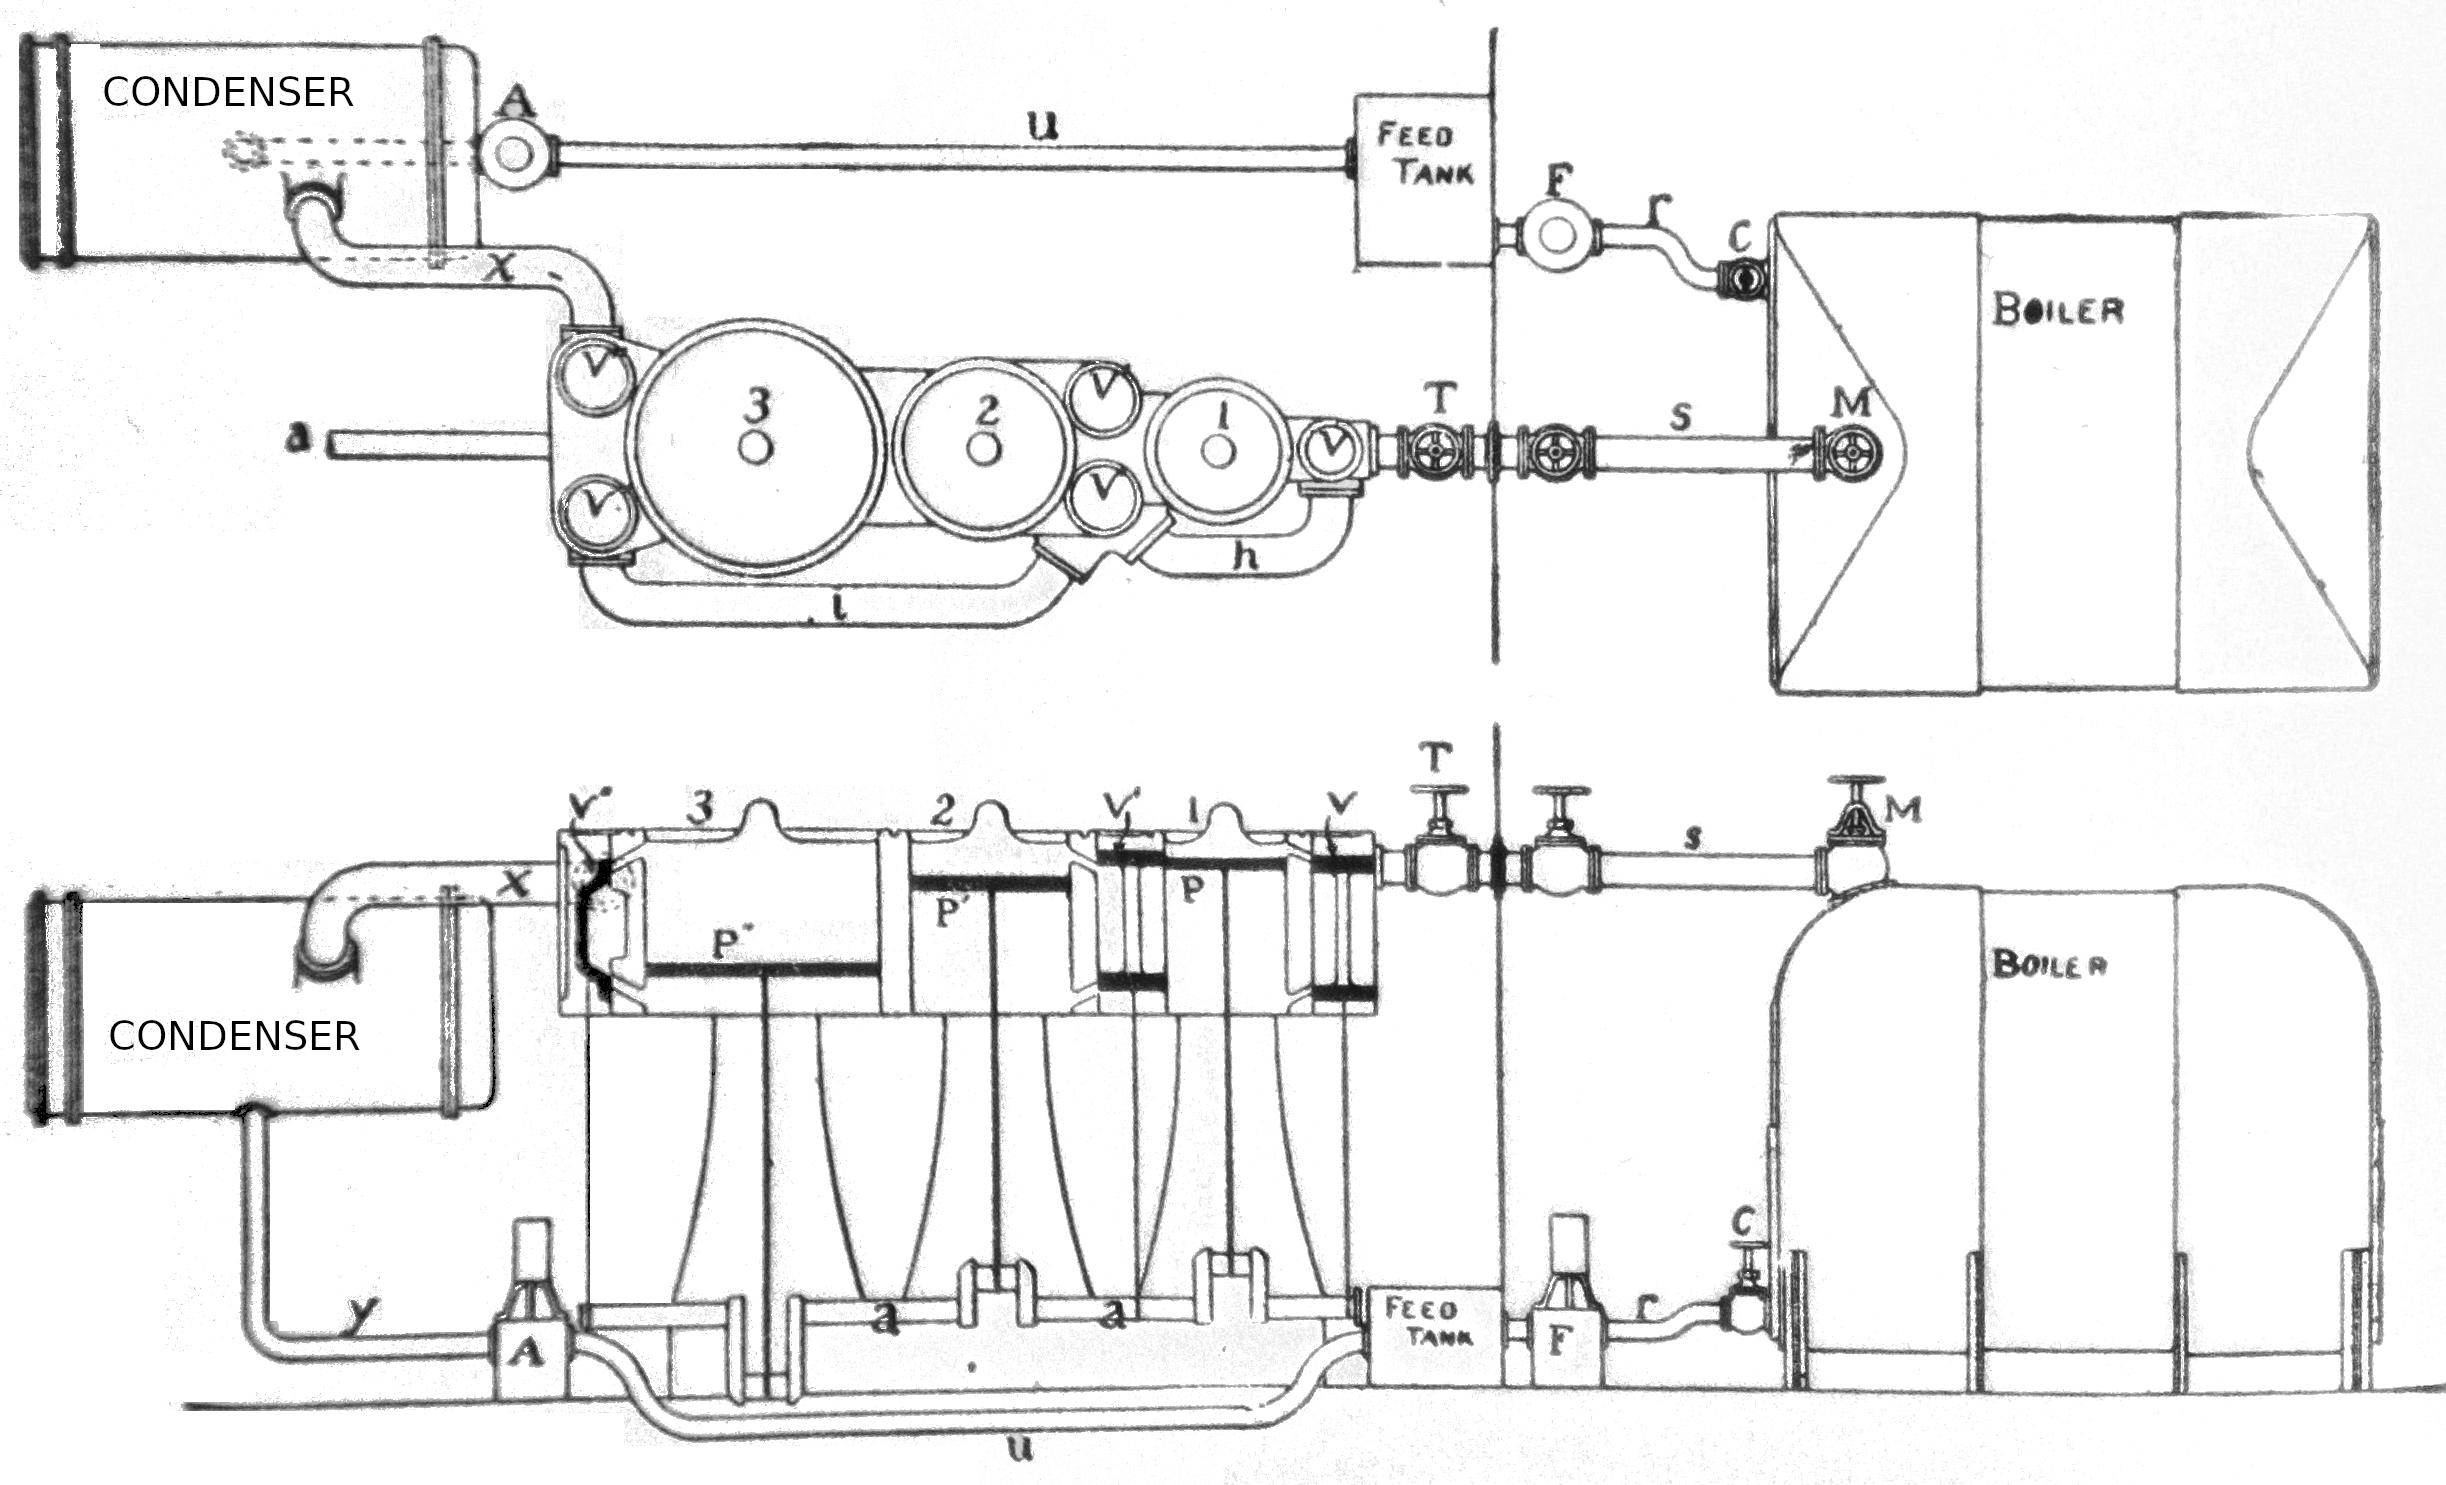
\includegraphics[scale=0.5]{fig_1.jpg}
  \caption*{\textsc{Fig.\ i.}}
\end{figure}

After acting on \textit{P} in one direction throughout its
\textit{stroke}, or distance that \textit{P} can travel in the
cylinder, the original quantity of steam is exhausted through one or
more additional cylinders into the \textit{condenser}, or it may be
exhausted from cylinder 1 direct into the condenser, or, more
directly, into the atmosphere.  In this last case, the engine is
called \textit{non-condensing}.\par

If only one cylinder and a condenser are used, they form a
\textit{simple condensing engine}.  When more than one is used, each
has its valve, piston, and other mechanism, the steam going through
the same action in each cylinder successively.  The cylinders, valves,
and pistons increase in size for each additional cylinder, and a
condenser is always used, the reasons for which will be shown later.
The pipes, \textit{h}, \textit{i} and other spaces connected the
exhaust side of one cylinder to the steam admission of th enext,
\textit{are called receivers}.\par

Engines in which hte steam passes successively through two, three, or
four cylinders are called \textit{double}, \textit{triple}, and
\textit{quadruple} expansion engines, the first one being commonly
called a \textit{compound} engine.  The cylinder which receives the
boiler steam is called the \textit{high-pressure} cylinder, and that
which exhausts it into the condenser, the \textit{low-pressure}
cylinder.  The cylinders between these two are called
\textit{intermediate-pressure} cylinders.  The various cylinders are
designated by the explanatory letters, H. P., I. P., and L.P\@.  For a
quadruple expansion engine, the I. P. cylinder next to the H. P. is
designated the 1st I. P., and the next one as the 2d I.P.\par

In the condenser, the steam is converted into water, which with any
air is removed by means of the \textit{air pump A} and returned to the
boiler through a \textit{feed tank} and by the \textit{feed pump F}.\par

\end{document}
